\documentclass[12pt]{article}
\usepackage[papersize={8cm,14cm},margin={.5cm,.5cm}]{geometry}
\usepackage{common}
\usepackage{amssymb}
\begin{document}
\begin{problem}
\item[6.] $G$ 為 $\triangle{ABC}$ 的重心,且 $D$ 為 $\overline{BC}$ 中點,如圖(六)所示。以 $G$ 為圓心,$\overline{GD}$ 長為半徑作一圓 $G$,並作 $A$ 點到圓 $G$ 的兩切線段 $\overline{AE}$、$\overline{AF}$,其中 $E$、$F$ 為切點。若 $\angle B = 30^\circ$,$\angle C = 45^\circ$,則 $\angle BAE + \angle CAF$ 的度數為何?
  \begin{figure}[ht]
    \centering
    \vspace*{-1ex}
    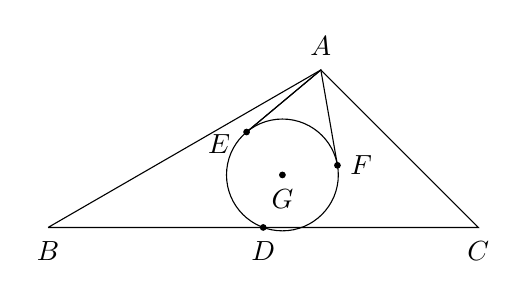
\begin{tikzpicture}
      \draw (-3.464,0) -- (2,0) -- (0,2) -- (-3.464,0);
      \filldraw (-.488,.667) circle (1pt);
      \filldraw (-.732,0) circle (1pt);
      \draw (-.488,.667) circle (.71cm);
      \draw (-.943,1.212) -- (0,2);
      \filldraw (-.943,1.212) circle (1pt);
      \draw (-.943,1.212) -- (0,2) -- (.211,.789);
      \filldraw (.211,.789) circle (1pt);
      \node at (0,2.3) {$A$};
      \node at (-3.464,-.3) {$B$};
      \node at (2,-.3) {$C$};
      \node at (-.732,-.3) {$D$};
      %\node at (-.763,.972) {$E$};
      \node at (-1.293,1.062) {$E$};
      \node at (.511,.789) {$F$};
      \node at (-.488,.367) {$G$};
    \end{tikzpicture}
    \vspace*{-1ex}
    \caption*{圖(六)}
    \vspace*{-2ex}
  \end{figure}
  \begin{choices}
    \item 40
    \item 45
    \item 50
    \item 55
  \end{choices}
\end{problem}
\end{document}
